\section{Homework 5}
\subsection{Exercise 4.15}

Relaxation of a boolean LP

A boolean linear program is defined as 
\begin{align}
  \text{minimize} & \quad c^T x \\
  \text{subject to} & \quad Ax \preceq b \\
  & \quad x_i \in \{ 0,1\}, i = 1, \dots, n 
\end{align}
This linear program can be relaxed by replacing the integer constraint with linear inequalities
\begin{align}
  \text{minimize} & \quad c^T x \\
  \text{subject to} & \quad Ax \preceq b \\
  & \quad 0 \leq x_i \leq 1, i = 1,\dots,n
\end{align} 
\subsubsection{Part a}
The optimal value of the LP relaxation is a lower bound on the optimal value. We can use a geometric example to prove this. Since the affine constraints in both the relaxed and original LP form a polyhedron. There are distinct vertex that either do or don't coincide with an integer point. In the event that the polyhedron's vertices land on the integer point, then if the optimal value lies on that vertex, then the optimal value for both the relaxed problem and original problem are equal. In the event that the vertex does not lie on the integer point, then the solution to the relaxed LP is a lower bound on the optimal value of the boolean LP.  \\ \\
The image below illustrates how the vertices lie on integers and therefore the optimal values would be equal. However, if the polyhedron extended out a bit to $(0,0.5),(0.5,0)$ as opposed to $(0,1),(1,0)$ then the relaxed polyhedron would be a strict lower bound.
\begin{figure}[htbp]
  \centerline{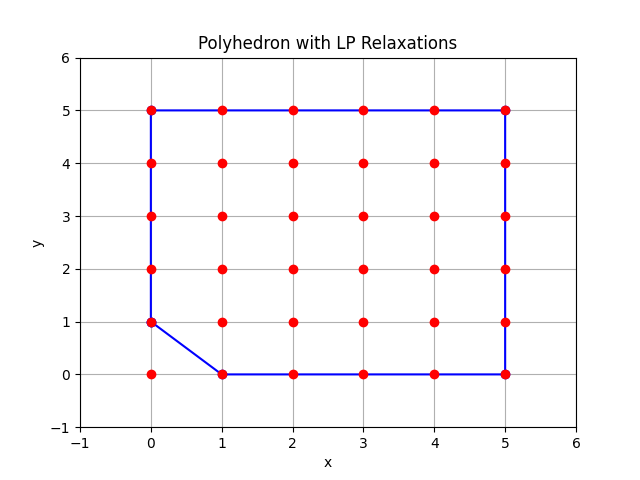
\includegraphics[width=0.75\textwidth]{hw5/lp_relaxed_polyhedron.png}}
  \caption{A polyhedron in $\mathbb{R}^2$ with points at each integer}
  \label{fig:lp_relaxed_polyhedron}
\end{figure} 
\subsubsection{Part b}
This section was also answered in part a. However, the solutions for the relaxation and original problem will coincide whenever the polyhedron created by the given $A$ and $b$ lie on an integer.